\section{模板工程专项安全施工方案}
\subsection{编制依据}

(1) 《建筑工程施工质量验收统一标准》(GB50300-2001)

(2) 《建筑结构荷载规范》(GB50009-2001)

(3) 《建筑施工模板安全技术规范》(JGJ162-2008)

(4) 《建筑施工扣件式钢管脚手架安全技术规范》(JGJ130-2011)

(5) 《建筑施工脚手架安全技术统一标准》(GB51210-2016)

(6) 《建筑施工安全检查标准》(JGJ59-2011)

(7) 《混凝土结构工程施工及验收规范》(GB50204-2015) 

\subsection{模板支撑架搭设要求}

(1) 必须设置纵横扫地杆。纵向扫地杆应采用直角扣件固定在距底座上皮不大于200mm 处的立杆上,
横向扫地杆也应采用直角扣件固定在紧靠纵向扫地杆下方的立杆上。当立杆基础不在同一高度上时,必须将高出的纵向扫地杆向低处延长两跨与立杆固定,高低差不应大于 1m。

(2) 立杆应采用对接接头,且接头位置不应设置在同一步内,同一步立杆的两个相隔接头在高度方向错开的距离不宜小于 500,
各接头中心至柱节点的距离不宜大于步距的 1/3。

(3) 纵向水平杆接长宜采用对接扣件连接,对接扣件应交错布置,两根相邻纵向水平杆接头不宜设置在同步或同跨内,
不同步或不同跨两个相邻接头在水平方向错开的距离不应小于 500m,各接头中心至最近主节点的距离不宜大于纵距的 1/3。

(4) 搭接长度不应小于 1m,应等距离设置 3 个旋转扣件固定,端部扣件盖板边缘至搭接纵向水平杆端的距离不应小于 100mm。

\subsection{模板计算书}
\subsubsection{基本参数}

(1) 钢筋混凝土板厚 $120mm$,板的模板采用木胶合板厚 $15mm$,面板下次愣采用 $40\times 80mm$ 木方,间距 $300mm$,主楞采用 $60\times 100mm$ ,木方间距 $500mm$,支撑体系采用 $\phi 48.3\times 3.6mm$ 钢管。

(2) 梁尺寸 $300\times 700mm$,模板采用木胶合板厚 $18mm$,侧模次楞采用 $40\times 80mm$ 木方, 布置间距 $200mm$,采用 $M20$ 对拉螺栓加固,
间距为 $250mm$,梁底次楞采用 $40\times 80mm$ 木方,次楞间距 $150mm$,梁模板主楞采用 $40\times 80mm$ 木方,间距 $500mm$,支撑体系采用 $Φ48.3\times 3.6mm$ 钢管。

(3) 柱尺寸 $500\times 500mm$ ,计算高度取 $9.0m$,模板采用木胶合板厚 $18mm$,次楞采用 $40\times 80mm$ 木方,间距为 $115mm$,
柱箍间距 $400mm$,最下一层柱箍距柱根间距为 $200mm$,最上一层柱箍距柱顶间距为 $200mm$,柱箍螺栓采用 $M18$。

\subsubsection{模板安全性验算}

(1) 对板的安全性验算\\

\quan{1} 楼板验算\\

根据《建筑结构荷载规范》(GB50009-2012),查得相关构件的标准荷载值如下:

模板自重标准值取 $G_{1k}=0.5 kN/m^2$

混凝土自重标准值取 $G_{2k}=24\times 0.12=2.88 kN/m^2 $

钢筋自重标准值取 $G_{3k}=1.1\times 0.12=0.132 kN/m^2$

施工活荷载标准值取 $2.5kN$($2.5kN/m$)

当活荷载作为均布线性荷载控制时:

\[q_1=0.9\times 1.0\times [1.2(500+2880+132)+1.4\times 2500]=6942 N/m\]

当恒荷载作为均布线性荷载控制时:

\[q_1=0.9\times 1.0\times [1.35(500+2880+132)+0.7\times 1.4\times 2500]=6471 N/m\]

$q$ 取较大值,故 $q=6942 N/m$

当作为集中荷载控制时:

\begin{align*}
    q_2&=0.9\times 1.0\times 1.2\times (500+2880+132)=3792 N/m\\
    P&=0.9\times 1.0\times 1.4\times 2500=3150N
\end{align*}

施工荷载为均布线荷载时的弯矩值为:

\begin{align}
    \label{fx:5.0}
    M_1=0.1ql^2=0.1\times 6.942\times 0.32=0.06kN\cdot m
\end{align}

施工荷载为集中荷载时的弯矩值为:

\begin{align}
    M_2&=0.1ql^2+0.213pl\\
    &=0.1\times 3.79\times 0.32+0.213\times 3.15\times 0.3 \notag\\
    &=0.23 kN \cdot m \notag
\end{align}

弯矩取最大值计算,故 $M=0.23kN\cdot m$\\

对板做强度验算,按照三跨连续梁计算,计算简图如下:

\begin{figure}[thbp!]
    \centering
    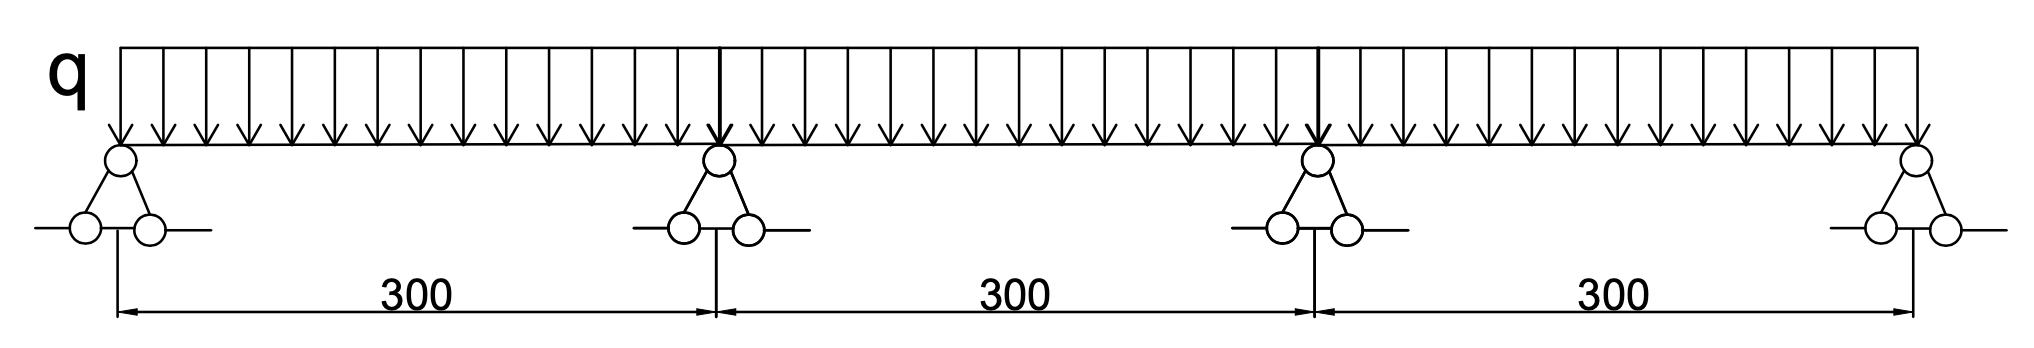
\includegraphics[width=1.0\linewidth]{figure/c5f1.png}
    \caption{楼板模板受力简图}
    \label{fig:c5f1}
\end{figure}


\begin{align}
    \label{fx:5.1}
    \sigma =\frac{M}{W}
\end{align}

式中,$M$ 为模板受到最大弯矩值;$W$ 为截面模量,矩形的截面模量公式为:

\begin{align}
    \label{fx:5.2}
    W=bh^2/6
\end{align}

式中,$b$ 为模板计算宽度;$h$ 为模板厚度。代入数据可得:

\begin{align*}
    W&=1000\times 152/6=37500 mm^3\\
    \sigma &=230000/37500=6.1 N/mm2<f=22 N/mm^2
\end{align*}

故板的强度满足要求。\\

对板做挠度验算,按照三跨连续梁计算,

\[q=0.9\times 1.0\times (500+2880+132)=3002 N/m\]

\begin{align}
    \label{fx:5.3}
    V_{max}=\frac{0.990ql^4}{100EI}
\end{align}

$E$ 为模板的弹性模量,取 $E=10000 N/mm^2$;$I$ 为截面惯性矩,计算公式为:

\begin{align}
    \label{fx:5.4}
    I=\frac{bh^3}{12}
\end{align}

代入数据得 $I=1000\times 15^3/12=281250 mm^4$。将截面惯性矩代入公式 \ref{fx:5.3} 得

\begin{align*}
    V&=\frac{0.99\times (3.002\times 10^2\times 300\times 10^2)}{100\times 10000\times 281250}\\
    &=0.058 mm < [v]=1/400=0.75 mm
\end{align*}

故板的挠度满足要求。\\

\quan{2} 板的次楞验算\\

板次楞采用 40×80mm 木方,间距 300mm,主楞间距 500mm。次楞的荷载按三跨连续梁计算受力,受理简图如下:

\begin{figure}[thbp!]
    \centering
    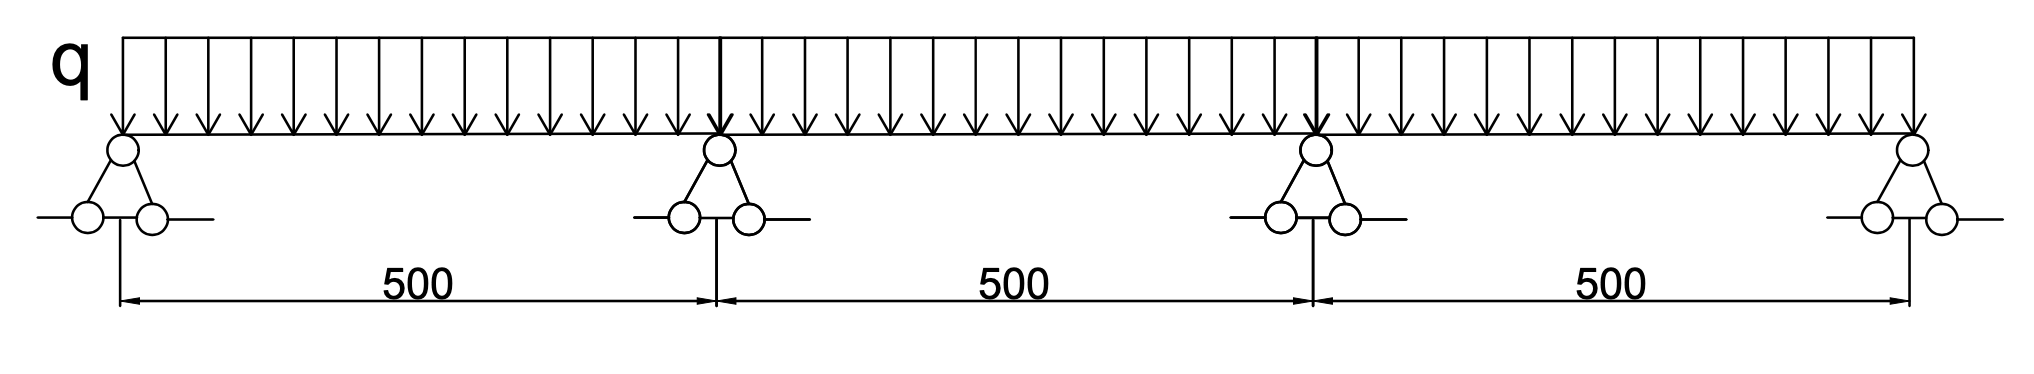
\includegraphics[width=1.0\linewidth]{figure/c5f2.png}
    \caption{板次楞受力简图}
    \label{fig:c5f2a}
\end{figure}


对板的次楞做强度验算:

\begin{align*}
    q_1&=0.9\times [1.2(500+2880+132)+1.4\times 2500]\times 0.3=1972 N/m \\
    q_2&=0.9\times (500+2880+132)\times 0.3=1.00 N/m
\end{align*}

分别按照公式 \ref{fx:5.0}、\ref{fx:5.2} 计算得出最大弯矩值与截面模量:

\begin{align*}
    M&=0.1\times 1.972\times 0.5^2=0.047 kN \cdot m\\
    W&=40\times 80^2 /6=42667 mm^2
\end{align*}

随后按照公式 \ref{fx:5.1} 求出板的次楞的强度:

\[
    \sigma = \frac{47000}{42667}=1.112 N/mm^2< f=17N/mm^2
\]

故次楞的强度满足要求。\\

对板的次楞做挠度验算,根据公式 \ref{fx:5.4} 算出次楞的最大截面惯性矩 $I$

\[
    I=40\times 80^3 /12=1706667 mm^4
\]

再将结果代回公式 \ref{fx:5.3},便可求出次楞的挠度设计值:

\begin{align*}
    V&=\frac{0.99\times 1 \times 500^4}{100\times 10000\times 1706667}\\
    &=0.0204 mm<[v]=1/400=1.25mm
\end{align*}

故次楞的挠度也满足要求。\\

\quan{3} 板的主楞验算\\

主楞采用 $60\times 100mm$ 木方,间距 $500mm$,板支撑在主楞上间距 $900mm$。由于木楞自重较小,因此计算时将其忽略
,主楞按照三跨梁计算,对主楞做强度验算:

\begin{align*}
    q_1&=0.9\times [1.2(500+2880+132)+1.4\times 2500]\times 0.5=3781 N/m \\
    q_2&=0.9\times (500+2880+132)\times 0.5=1.58 N/m
\end{align*}

按照主楞的最大弯矩公式求出主楞的最大弯矩值:

\begin{align}
    M=0.289q_1l=0.289\times 3.78\times 0.9=0.98 kN \cdot m
\end{align}

按照公式\ref{fx:5.2} 计算得出主楞的截面模量:

\[
    W=60\times 100^2 /6=100000 mm^2
\]

随后按照公式 \ref{fx:5.1} 求出板的主楞的强度:

\[
    \sigma = \frac{980000}{100000}=9.8 N/mm^2< f=17N/mm^2
\]

故主楞的强度满足要求。\\

对板的主楞做挠度验算,根据公式 \ref{fx:5.4} 算出次楞的最大截面惯性矩 $I$

\[
    I=60\times 100^3 /12=5000000 mm^4
\]

再将结果代回公式 \ref{fx:5.3},便可求出次楞的挠度设计值:

\begin{align*}
    V&=\frac{0.99\times 1580 \times 900^3}{100\times 10000\times 5000000}\\
    &=0.23 mm<[v]=1/400=2.25mm
\end{align*}

故主楞的挠度也满足要求。\\

\quan{4} 板的立杆验算\\

楼板支模高度 $9.0m$,属于高支模,立杆采用 $\phi 48.3\times 3.6$ 钢管,底部设置一道拉结杆,向上每 $1.5m$ 设置一道拉结杆。

查规范可得各个关键部件的自重标准值:

支撑自重为 $0.1444\times 9.0=1.29kN$

混凝土自重为 $24\times 0.12\times 0.5\times 0.9=1.29kN $

钢筋自重为 $1.1\times 0.12\times 0.5\times 0.9=0.05kN$

按照各个部件的自重标准值,能够求出恒荷载与活荷载的值:

恒荷载为 $1.27+1.29+0.05=2.63kN$

活荷载为 $2.5\times 0.5\times 0.9=1.125kN$

当活荷载控制时:

\[N_1=0.9\times (1.2\times 2.63+1.4\times 1.125)=4.25kN\]

当恒荷载控制时:

\[N_2=0.9\times (1.35\times 2.63+1.4\times 0.7\times 1.125=4.18kN\]

立杆轴向力取值取最大荷载值,即 $N=4.25 kN$

计算满堂脚手架的立杆长度的公式如下:

\begin{align}
\label{fx:5.5}
l_0&=k\mu_1(h+2a)\\
\label{fx:5.6}
l_0&=k\mu_2h
\end{align}

式中:
$k$ 为满堂支撑架立杆计算长度附加系数,取 1.185;   

$h$ 为步距 1.5m;                           

$a$ 为立杆伸出顶层水平杆中心线至支撑点长度 20mm;

$\mu_1$、$\mu_2$ 为满堂支撑架整体稳定因素的单杆计算长度系数,
根据《建筑施工扣件式脚手架安全技术规范》取值为 $\mu_1=1.54$、$\mu_2=1.951$

将上述数据代入公式 \ref{fx:5.5}、\ref{fx:5.6} 得:

\begin{align*}
    l_1&=1.185\times 1.54\times (1.5+2\times 0.2)=3.467 m\\
    l_2&=1.185\times 1.951\times 1.5=3.468 m
\end{align*}

$l_0$ 取二者最大值,即 $l_0=3.468 m$,随后根据公式 $\lambda=l_0/i$ 求出长细比为

\[
    \lambda = \frac{3.468}{1.59}=218
\]

查表可得轴心受压构件的稳定系数 $\phi =0.153$,再将上述所有数据代入下式可得出杆的弯曲正应力 $\sigma $

\begin{align}
\sigma &=\frac{N}{\phi A}\\
&=\frac{4180}{0.153\times 506} \notag\\
&=53.9 N/mm^2<f=205 N/mm^2 \notag
\end{align}

故主杆满足设计要求。\\

(2) 对梁的安全性验算\\

\quan{1} 梁模板计算\\

梁模板计算取首层截面尺寸最大的梁进行计算,截面尺寸为 300×700mm,模板采用 18mm
厚木模板,次楞间距 200mm。

\begin{figure}[thbp!]
    \centering
    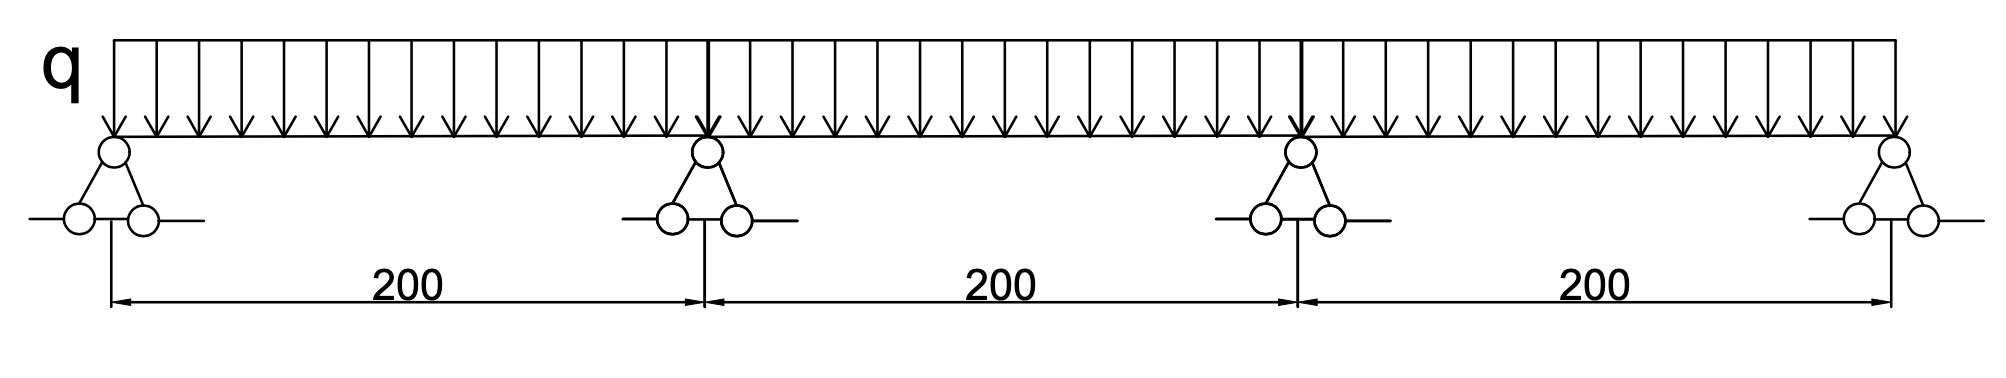
\includegraphics[width=1.0\linewidth]{figure/c5f3.png}
    \caption{梁侧模受力简图}
    \label{fig:c5f3}
\end{figure}

新浇混凝土作用于模板的侧压力,可以使用下列公式做计算:

\begin{align}
    \label{fx:5.7}
    F&=0.22\gamma_c t_0\beta_1 \beta_2V^{\frac{1}{2}}\\
    \label{fx:5.7a}
    F&=\gamma_c H
\end{align}

式中:

$\gamma_c$ 为混凝土重力密度,根据规范取值 $24 kN/m^3$;

$t_0$ 为混凝土入模温度,根据

\begin{align}
\label{fx:5.8}
t_0=\frac{200}{t+15}
\end{align}

可以计算出,$t$ 为当前温度;为方便计算,$t$ 取 20 摄氏度;

$\beta_1$ 为外加剂影响修正系数,根据规范取 1.0;

$\beta_2$ 为混凝土坍落度影响修正系数,根据规范取 1.0;

$V$ 为混凝土浇筑速度,根据计算手册,为方便取 $2 m/h$;

$H$ 混凝土侧压力计算位置至新浇筑混凝土顶面总高度为 700mm;

根据公式 \ref{fx:5.8} 、\ref{fx:5.7} 和 \ref{fx:5.7a} 分别可得 

    \begin{align*}
        t_0&=200/(20+15)=5.71\\
        F_1&=0.22\times 24\times 5.71\times 1\times 1\times 2^{\frac{1}{2}}=42.6 kN/m^2\\
        F_2&=24\times 0.7=16.8 kN/m^2
    \end{align*}

则新浇混凝土作用于模板的侧压力的标准值 $G_{4k}=16.8 kN/m^2$,查表得可变荷载标准值 $Q_{2k}=4 kN/m^2$,所以

当恒荷载做控制时

\[
    q_1=0.9\times 0.7\times (1.35\times 16.8+1.4\times 0.7\times 4)=15.5 kN/m
\]

当活荷载做控制时

\[
    q_1^{'}=0.9\times 0.7\times (1.2\times 16.8+1.4\times 4)=14.4 kN/m
\]

荷载组合强度取最大值 $15.5 kN/m$,荷载组合的挠度计算值为

\[
    q=0.9\times 0.7\times 16.8=10.05 kN/m
\]

对梁模板做强度验算,分别根据公式 \ref{fx:5.0}、\ref{fx:5.2} 计算得出最大弯矩值与截面模量:

\begin{align*}
    M&=0.1\times 15.5\times 200^2=620000 N \cdot mm\\
    W&=1000\times 18^2 /6=54000 mm^2
\end{align*}

随后按照公式 \ref{fx:5.1} 求出板的次楞的强度:

\[
    \sigma = \frac{62000}{54000}=1.1 N/mm^2< f=17N/mm^2
\]

故梁模板的强度满足要求。\\

对梁模板做挠度验算,根据公式 \ref{fx:5.4} 算出次楞的最大截面惯性矩 $I$

\[
    I=1000\times 18^3 /12=486000 mm^4
\]

再将结果代回公式 \ref{fx:5.3},便可求出次楞的挠度设计值:

\begin{align*}
    V&=\frac{0.99\times 10.05 \times 200^3}{100\times 10000\times 486000}\\
    &=0.3 mm<[v]=1/400=0.5mm
\end{align*}

故梁模板的挠度也满足要求。\\

\quan{2} 梁侧模次楞验算\\

梁侧次楞采用 40×80mm 木方,间距 200mm,主楞间距 500mm。木楞自重影响较小,计算时忽略不计,次楞的荷载按三跨连续梁计算受力,梁侧模次楞
受理简图如下:

\begin{figure}[thbp!]
    \centering
    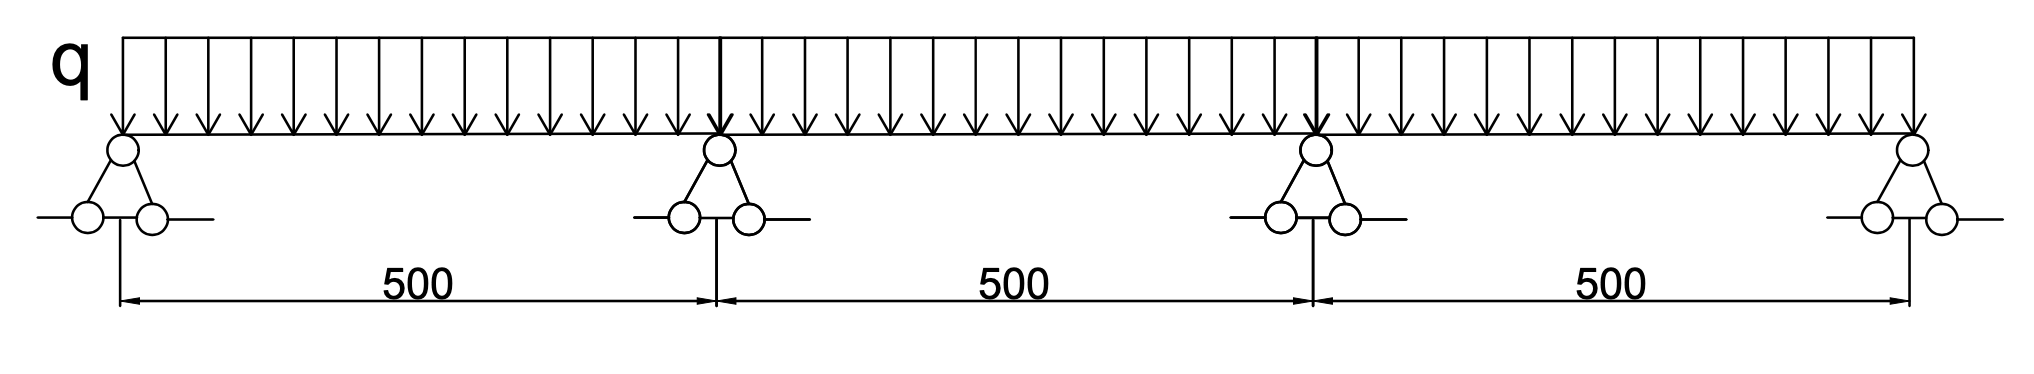
\includegraphics[width=1.0\linewidth]{figure/c5f2.png}
    \caption{梁侧模次楞受力简图}
    \label{fig:c5f2b}
\end{figure}

对板的次楞做强度验算:

\begin{align*}
    q_1&=0.9\times 0.2\times [1.35\times 1.68+1.4\times0.7\times 2]=4.43 kN/m \\
    q_2&=0.9\times 16.8\times 0.2=3.02 kN/m
\end{align*}

分别按照公式 \ref{fx:5.0}、\ref{fx:5.2} 计算得出最大弯矩值与截面模量:

\begin{align*}
    M&=0.1\times 4430\times 500^2=110000 N \cdot mm\\
    W&=40\times 80^2 /6=42667 mm^2
\end{align*}

随后按照公式 \ref{fx:5.1} 求出板的次楞的强度:

\[
    \sigma = \frac{110000}{42667}=2.6 N/mm^2< f=17N/mm^2
\]

故梁侧模次楞的强度满足要求。\\

对梁侧模的次楞做挠度验算,根据公式 \ref{fx:5.4} 算出次楞的最大截面惯性矩 $I$

\[
    I=40\times 80^3 /12=1706667 mm^4
\]

再将结果代回公式 \ref{fx:5.3},便可求出次楞的挠度设计值:

\begin{align*}
    V&=\frac{0.99\times 3.02 \times 500^4}{100\times 10000\times 1706667}\\
    &=0.264 mm<[v]=1/400=1.25mm
\end{align*}

故梁侧模的次楞的挠度也满足要求。\\

\quan{3} 侧模对拉螺栓验算\\

对拉螺栓采用 M12,水平间距 500mm,竖向间距 200mm,对拉螺栓最大轴力设计值可按以下公式求出:

\begin{align}
    \label{fx:5.9}
    N^b_t>N&=abF_s
\end{align}

式中 $a$、$b$ 分别为对拉螺栓的水平间距和竖向间距, $F_s$ 为新浇混凝土作用于模板上的侧压力、振捣混凝土对垂直模板产生的水平荷载或倾倒混凝土时作用于模板上的侧压力设计值:

\begin{align}
    \label{fx:5.9a}
    F_s=0.95(r_GF+r_QQ_{3k})
\end{align}

或者

\begin{align}
    \label{fx:5.9b}
    F_s=0.95(r_GG_{4k}+r_QQ_{3k})
\end{align}

其中 0.95 为荷载值折减系数,针对本项目应该使用公式 \ref{fx:5.9b},代入数据得

\[
F_s=0.95\times(1.35\times 16.8+1.4\times 2.0)=24.21 kN/m^2    
\]

将计算得出的 $F_s$ 代回 \ref{fx:5.9},得

\[N=0.2\times 0.5\times 24.21=2.42 kN\]

查表得 M12 对拉螺栓的 $N_t^b$ 值为 $12.9 kN$,因为 $2.42<12.9$,故对拉螺栓的设计值可以满足要求。\\

\quan{4} 梁底模验算\\

取 300 宽板计算,梁底设置 3 个 40×80 次楞,间距 150mm,受力简图如下:

\begin{figure}[thbp!]
    \centering
    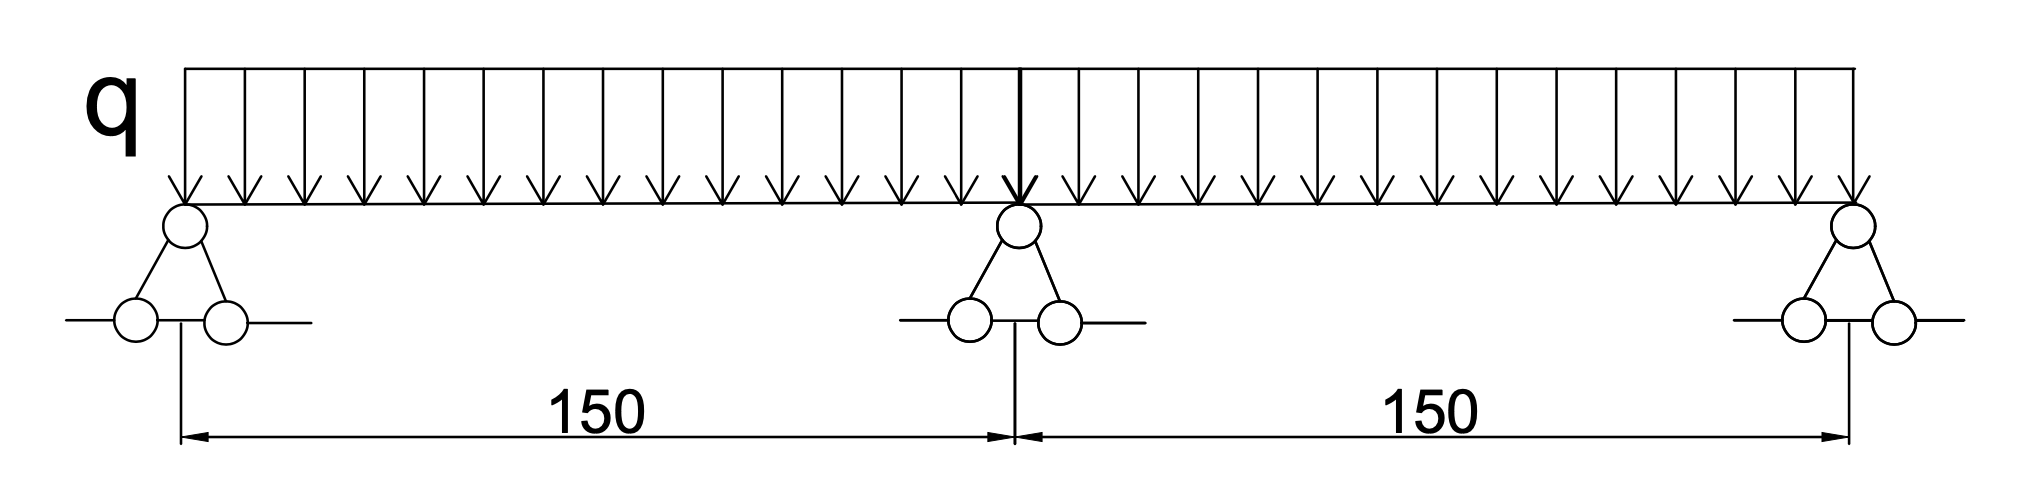
\includegraphics[width=0.7\linewidth]{figure/c5f4.png}
    \caption{梁底模板受力简图}
    \label{fig:c5f4}
\end{figure}

按照三跨连续板计算,根据《建筑结构荷载规范》(GB50009-2012),
查得相关构件的标准荷载值如下:

模板自重标准值取 $0.5 kN/m^2$

混凝土自重标准值取 $2.4\times 0.7=16.8 kn/m^2$

钢筋自重标准值取 $1.5\times 0.7=1.05 kN/m^2$

当由活荷载控制荷载时:

\[q_1=0.9\times 0.3\times[1.2\times(0.5+16.8+1.05)+1.4\times 2]=6.71 kN/m\]

当由恒荷载控制荷载时:

\[q_1^{'}=0.9\times 0.3\times[1.35\times(0.5+16.8+1.05)+1.4\times0.7\times 2]=7.2 kN/m\]

$q_1$ 取二者最大值,即 $7.2 kN/m$,$q_2=0.9\times 0.3\times (0.5+16.8+1.05)=4.9 kN/m$

对梁底模模板做强度验算,按照公式

\begin{align}
    \label{fx:5.X}
    M=0.096ql^2
\end{align}

可以计算得出截面的最大弯矩,按照公式\ref{fx:5.2} 可以计算得出截面模量:

\begin{align*}
    M&=0.096\times 7.2\times 150^2=15552 N \cdot mm\\
    W&=1000\times 18^2 /6=54000 mm^2
\end{align*}

随后按照公式 \ref{fx:5.1} 求出梁底模模板的强度:

\[
    \sigma = \frac{15552}{54000}=0.28 N/mm^2< f=17N/mm^2
\]

故梁底模模板的强度满足要求。\\

对梁侧模的次楞做挠度验算,根据公式 \ref{fx:5.4} 算出次楞的最大截面惯性矩 $I$

\[
    I=1000\times 18^3 /12=486000 mm^4
\]

再将结果代回公式 \ref{fx:5.3},便可求出梁底模模板的挠度设计值:

\begin{align*}
    V&=\frac{0.99\times 4.9 \times 150^4}{100\times 10000\times 486000}\\
    &=0.005 mm<[v]=1/400=0.3mm
\end{align*}

故梁底模模板的挠度也满足要求。\\

\quan{5} 梁底模次楞验算\\

梁底模次楞采用 40×80mm 木方,间距 150mm,主楞间距 500mm。木楞自重影响较小,计算时忽略不计,次楞的荷载按三跨连续梁计算受力,
受理简图如下:

\begin{figure}[thbp!]
    \centering
    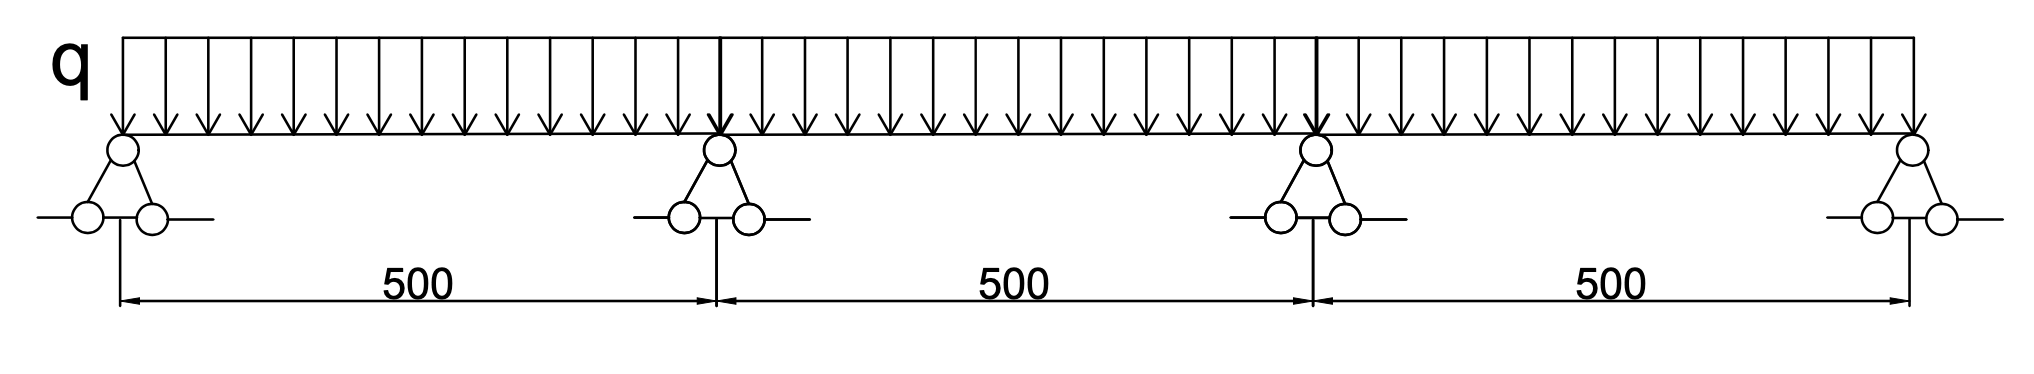
\includegraphics[width=1.0\linewidth]{figure/c5f2.png}
    \caption{梁底模次楞受力简图}
    \label{fig:c5f2c}
\end{figure}

当荷载由活荷载控制时:

\[q_1=0.9\times 0.15\times [1.2\times (0.5+16.8+0.15)+1.4\times 2]=3.20 kN/m\]

当荷载由恒荷载控制时:

\[q_1=0.9\times 0.15\times [1.35\times (0.5+16.8+0.15)+1.4\times0.7\times 2]=3.44 kN/m\]

$q_1$ 取二者最大值,即 $3.44 kN/m$,$q_2=0.9\times 0.15\times (0.5+16.8+0.15)=2.3 kN/m$

分别按照公式 \ref{fx:5.0}、\ref{fx:5.2} 计算得出最大弯矩值与截面模量:

\begin{align*}
    M&=0.1\times 3440\times 500^2=86000 N \cdot mm\\
    W&=40\times 80^2 /6=42667 mm^2
\end{align*}

随后按照公式 \ref{fx:5.1} 求出梁底模次楞的强度:

\[
    \sigma = \frac{86000}{42667}=2.02 N/mm^2< f=17N/mm^2
\]

故梁底模次楞的强度满足要求。\\

对梁底模次楞做挠度验算,根据公式 \ref{fx:5.4} 算出梁底模次楞的最大截面惯性矩 $I$

\[
    I=40\times 80^3 /12=1706666 mm^4
\]

再将结果代回公式 \ref{fx:5.3},便可求出次楞的挠度设计值:

\begin{align*}
    V&=\frac{0.99\times 2.30 \times 500^4}{100\times 10000\times 1706666}\\
    &=0.05 mm<[v]=1/400=1.25mm
\end{align*}

故梁底模次楞的挠度也满足要求。\\

\quan{6} 梁底模主楞验算\\

梁底模主楞采用 40x80mm 木方,间距 500mm,支撑在主楞上间距 300mm,由于木楞的自重对结构的影响较小,
故计算时忽略木楞自重,梁底主楞按照单跨简支梁计算,由活荷载做控制,受力简图如下:

\begin{figure}[thbp!]
    \centering
    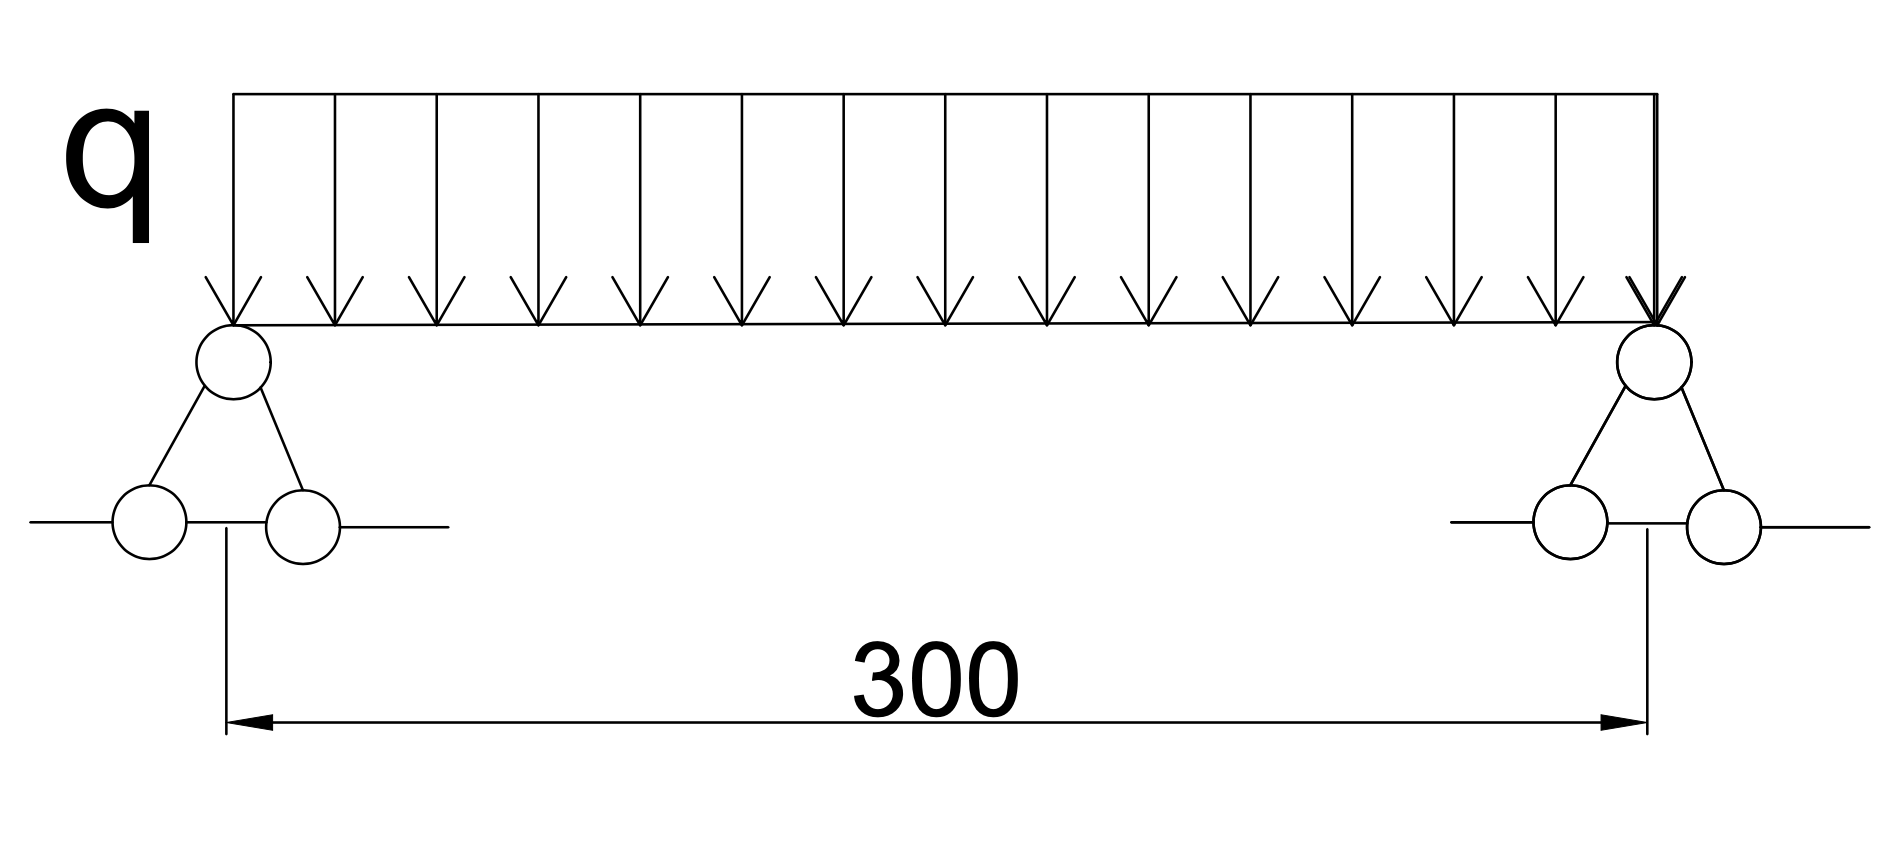
\includegraphics[width=0.5\linewidth]{figure/c5f5.png}
    \caption{梁底模主楞受力简图}
    \label{fig:c5f5}
\end{figure}

\begin{align*}    P_1&=\frac{3550\times 0.3}{2}=0.53 kN\\
    P_2&=\frac{2300\times 0.3}{2}=0.34 kN
\end{align*}

对梁底模主楞做强度验算,按照公式

\begin{align}
    \label{fx:5.A}
    M=\frac{1}{4}p_1l
\end{align}

可以计算得出截面的最大弯矩,按照公式 \ref{fx:5.2} 可以计算得出截面模量:

\begin{align*}
    M&=\frac{1}{4}\times 0.53\times 0.3=40000 N \cdot mm\\
    W&=40\times 80^2 /6=42666 mm^2
\end{align*}

随后按照公式 \ref{fx:5.1} 求出梁底模主楞的强度:

\[
    \sigma = \frac{40000}{42666}=1.0 N/mm^2< f=17N/mm^2
\]

故梁底模主楞的强度满足要求。\\

对梁底模主楞做挠度验算,根据公式 \ref{fx:5.4} 算出梁底模主楞的最大截面惯性矩 $I$

\[
    I=40\times 80^3 /12=1706666 mm^4
\]

再将结果代回简支梁最大挠度公式 

\begin{align}
    V_{max}&=\frac{5p_2l^3}{384EI}\\
    &=\frac{5\times 340\times 300^3}{384\times 10000\times 170666} \notag \\
    &=0.07mm<[v]=1/400=0.75mm \notag
\end{align}

便可求出梁底模主楞的挠度也满足要求。\\

(3) 对柱的安全性验算\\

\quan{1} 柱箍间距计算

柱选取首层截面尺寸最大的柱进行计算,截面尺寸为 500×500mm,计算高度 9.0m, 模板采用 18mm 厚木模板,竖楞采用 40×80mm 木方,
间距 100mm,用柱箍固定,柱箍处用 M18 螺栓加固。受力简化为三跨简支梁,简图如下:

当柱模板为木面板时柱箍间距应按照如下公式计算:

\begin{align}
    \label{fx:5.B}
    L \leq 0.783\sqrt[3]{\frac{EI}{Fb}}
\end{align}

式中 $L$ 为柱箍间距,$E$ 为面板的弹性模量,取 10000,$b$ 为面板宽度,为 500mm,根据公式 \ref{fx:5.4} 可求出 $I$ ,
根据公式 \ref{fx:5.7} 可以求出式中的 $F$:

\begin{align*}
I&=\frac{500\times 18^3}{12}=243000\\
F&=0.22\times 24\times 5.71\times 1\times 1\times 2^{\frac{1}{2}}=42600 N/mm^2
\end{align*}

将上述所有数值代回公式 \ref{fx:5.B} 可得出柱箍间距 $L$ 为

\[L \leq 0.783\times \sqrt[3]{\frac{10000\times 243000}{4260000\times 10^{-6}\times 500}}=399mm\]

此外,柱箍间距还应满足

\begin{align}
    \label{fx:5.C}
    L \leq \sqrt{\frac{8Wf_m}{F_sb}}=\sqrt{\frac{8\times 27000\times 35}{42600\times 10^{-6}\times 500}}=595 mm
\end{align}

比较这两个结果,二者取最小值,即柱箍间距 $L=400mm$。

\quan{2} 柱模板安全验算

墙体模板受力可以简化为三跨梁连续梁,受力简图如下:

\begin{figure}[thbp!]
    \centering
    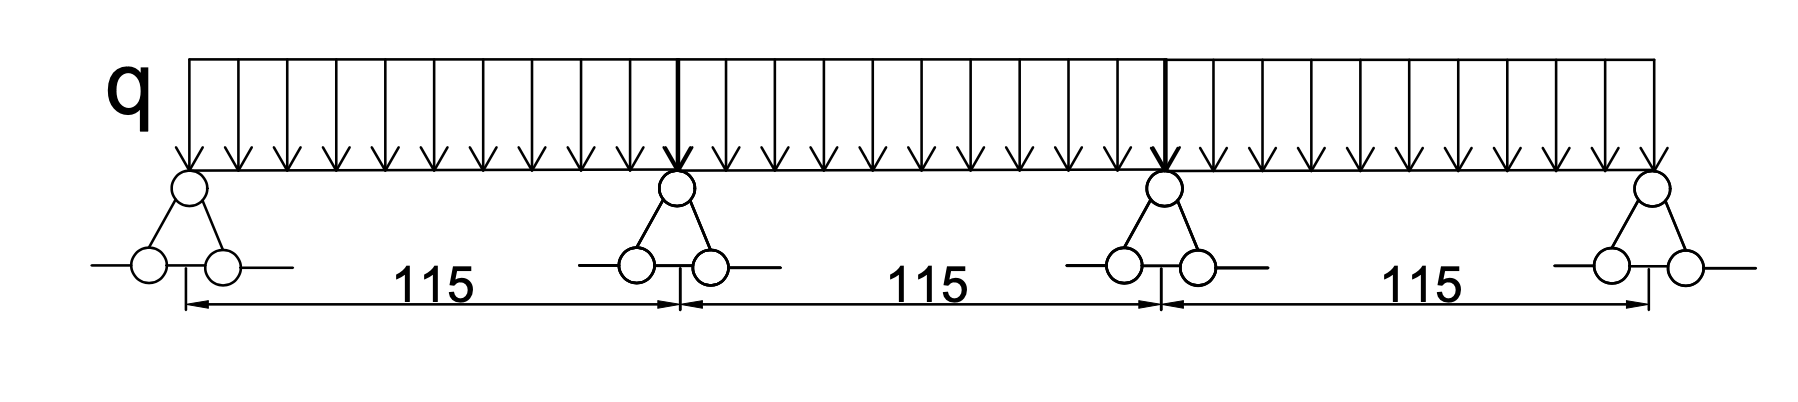
\includegraphics[width=1.0\linewidth]{figure/c5f6.png}
    \caption{墙体模板受力简图}
    \label{fig:c5f6}
\end{figure}

根据公式 \ref{fx:5.7} 和 \ref{fx:5.7a} 可以求出新教混凝土作用于模板上的侧压力设计值 $G_{4k}$

\begin{align*}
    F_1&=0.22\times 24\times 5.71\times 1\times 1\times 2^{\frac{1}{2}}=42600 N/mm^2\\
    F_2&=\times 9000=216 kN/m^2
\end{align*}

二者取较小值,则新教混凝土作用于模板上的侧压力设计值 $G_{4k}=42.6 kN/m^2$,按照规范取钢筋自重标准值 $G_{3k}=2kN/m^2$

当活荷载做控制时

\[q_1=0.9\times 0.5\times (1.2\times 42.6+1.4\times 2)=22.7kN \cdot m\]

当恒荷载做控制时

\[q_1^{'}=0.9\times 0.5\times (1.35\times 42.6+1.4\times 0.7\times 2)=26.7kN \cdot m\]

$q_1$ 取二者最大值,即 $26.7 kN/m$,$q_2=0.9\times 42.6=38.34 kN/m$

分别按照公式 \ref{fx:5.0}、\ref{fx:5.2} 计算得出最大弯矩值与截面模量:

\begin{align*}
    M&=0.1\times 26.7\times 100^2=26700 N \cdot mm\\
    W&=100\times 18^2 /6=54000 mm^2
\end{align*}

随后按照公式 \ref{fx:5.1} 求出柱模板的强度:

\[
    \sigma = \frac{54000}{26700}=2.02 N/mm^2< f=17N/mm^2
\]

故柱模板的强度满足要求。\\

对柱模板做挠度验算,根据公式 \ref{fx:5.4} 算出柱模板的最大截面惯性矩 $I$

\[
    I=500\times 18^3 /12=243000 mm^4
\]

再将结果代回公式 \ref{fx:5.3},便可求出柱模板的挠度设计值:

\begin{align*}
    V&=\frac{0.99\times 38.3 \times 100^4}{100\times 10000\times 486000}\\
    &=0.15 mm<[v]=1/400=1.25mm
\end{align*}

故柱模板的挠度也满足要求。\\

\quan{3} 柱竖楞验算

柱竖楞的荷载按三跨连续梁计算受力,计算简图如下:

\begin{figure}[thbp!]
    \centering
    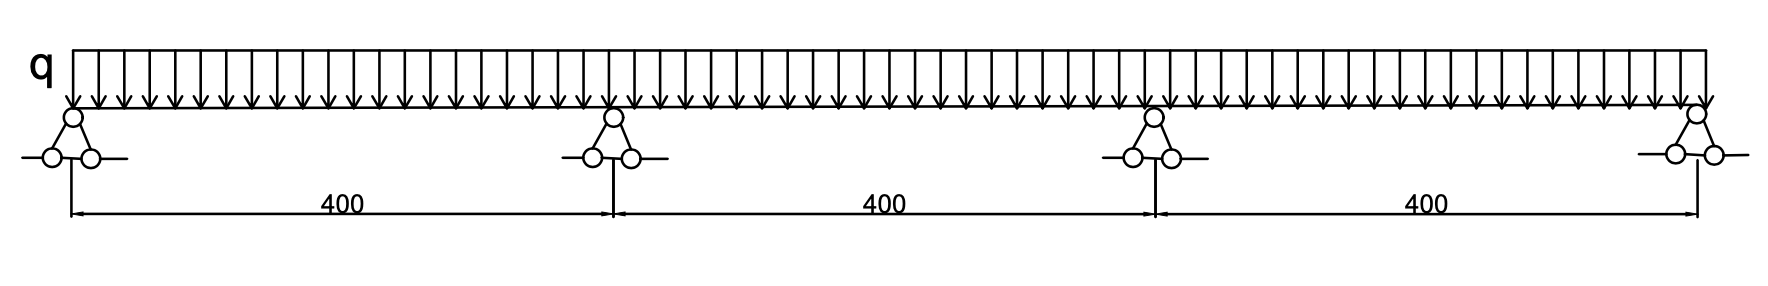
\includegraphics[width=1.0\linewidth]{figure/c5f7.png}
    \caption{柱竖楞受力简图}
    \label{fig:c5f7}
\end{figure}

\begin{align*}
    q_1&=0.9\times 0.1\times(1.35\times 42.6+1.4\times 0.7\times 2)=5.4 kN/m\\
    q_2&=0.9\times 0.1\times 42.6=3.83 kN/m
\end{align*}

分别按照公式 \ref{fx:5.0}、\ref{fx:5.2} 计算得出最大弯矩值与截面模量:

\begin{align*}
    M&=0.1\times 5400\times 500^2=86000 N \cdot mm\\
    W&=40\times 80^2 /6=42667 mm^2
\end{align*}

随后按照公式 \ref{fx:5.1} 求出柱竖楞的强度:

\[
    \sigma = \frac{86000}{42667}=2.02 N/mm^2< f=17N/mm^2
\]

故柱竖楞的强度满足要求。\\

对柱竖楞做挠度验算,根据公式 \ref{fx:5.4} 算出柱竖楞的最大截面惯性矩 $I$

\[
    I=40\times 80^3 /12=1706666 mm^4
\]

再将结果代回公式 \ref{fx:5.3},便可求出柱竖楞的挠度设计值:

\begin{align*}
    V&=\frac{0.99\times 3.83 \times 400^4}{100\times 10000\times 1706666}\\
    &=0.56 mm<[v]=1/400=1.25mm
\end{align*}

故柱竖楞的挠度也满足要求。\\

\quan{4} 柱箍验算

柱箍采用 40x80mm 的木材质,按照简支梁计算,使用公式 \ref{fx:5.D} 求得柱箍强度:

\begin{align}
    \label{fx:5.D}
    \frac{N}{A_n}+\frac{M_x}{W_nx}\leq f \ \text{或} \ (f_m)
\end{align}

其中

\begin{align}
\label{fx:5.E}
N&=\frac{1}{2}ql_3\\
&=0.5\times 17040\times 05=4040 N \notag\\
\label{fx:5.F}
q&=F_sl_1\\
&=42600\times 0.4=17040 N/mm \notag\\
\label{fx:5.G}
M_x&=\frac{ql_2^2}{8}=\frac{F_sl_1L_2^2}{8}\\
&=\frac{17040\times (500+15\times 2)}{8}=598317 N \cdot mm \notag
\end{align}

在公式 \ref{fx:5.D} 中的柱箍截面面积 $A_n=40\times 80=3200 mm^2$;柱箍界面抵抗矩 $W_{nx}=80^2\times 40/6=42666 mm^3$
将上述数据代回公式 \ref{fx:5.D} 中得

\begin{align*}
    \frac{N}{A_n}+\frac{M_x}{W_nx}=\frac{4040}{3200}+\frac{598317}{42666}=15.28 N/mm^2
\end{align*}

查表得 $f_m=17N/mm^2$,$15.28<17N/mm^2$ 故强度满足要求。

对柱箍做挠度验算,$q_2=\times 0.9\times 42.6\times 0.4=15.3 N/mm^2$,
根据公式 \ref{fx:5.4} 算出柱箍的最大截面惯性矩 $I$

\[
    I=40\times 80^3 /12=1706666 mm^4
\]

再按照简支梁计算公式将结果代回

\begin{align*}
    V_{max}&=\frac{5q_2l^3}{384EI}\\
    &=\frac{5\times 15.3\times (500+15\times 2)^3}{384\times 10000\times 170666}\\
    &=0.92mm<[v]=1/400=1.225mm
\end{align*}

便可求出柱箍的挠度也满足要求。\\

\quan{5} 螺栓验算

螺栓采用 M18,竖向间距 400mm。根据公式 \ref{fx:5.9} 、\ref{fx:5.9b} 可得

\begin{align*}
    F_s&=0.95\times(1.2\times 42.6+1.4\times 2)=51.2 kN/m^2
    N&=0.5\times 0.3\times 51.2=7.68 kN
\end{align*}

查表得 M18 螺栓的 $N^b_t$ 值为 $29.6 kN>7.68 kN$,故螺栓满足设计要求。

\subsection{模板安装及拆除}
\subsubsection{模板安装}

(1) 模板安装前应该审查模板结构设计说明书,确保手续齐全

(2) 应进行全面的安全技术交底,操作班组应该熟悉设计与施工说明书,并做好模板安装作业的分工准备

(3) 模板安装应该按照设计与施工说明书按顺序拼装。木杆、钢管、门架等支架立柱不得混用

(4) 竖向模板和支架立柱支撑部分安装在基土之上时,应加设垫板,垫板应有足够的强度和支承面积,且应中心承载,基土应坚实,并附有排水措施

(5) 模板及其支架在安装过程中必须设立有效的防止倾覆的临时固定设施

(6) 现浇钢筋混凝土梁板当跨度大于 4 米时,模板应起拱。

(7) 模板应有足够的承载能力,刚度和稳定性。

(8) 楼板模板施工前应先弹线,根据弹线搭设脚手架,先搭设梁底然后搭设板底,调整梁底钢管标高,调平后,铺设梁底模,梁底模两侧用扣件锁紧,防止梁底模跑位; 

(9) 梁钢筋绑扎完毕后,封梁侧模,梁侧模应落在梁底模上,梁模板转角处必须设置木方; 

(10) 铺设主次龙骨,模板拼缝要严密,用对拉螺栓固定模板, 楼板模板压在梁侧模上。

\subsubsection{模板拆除}

(1) 模板拆除应该经过相关管理人员的批准,按照国家标准《混凝土结构工程施工质量验收规范》(GB50204)的有关规定执行;

(2) 当混凝土未达规定强度,或已经达到规定强度,但需提前拆模的,必须经过计算和主管部门的批准后方可拆除;

(3) 大体积混凝土的拆模时间除了要满足混凝土强度要求之外,还应使得混凝土内外温差降低到 25 摄氏度以下时方可拆模;

(4) 拆模前应确定所使用的工具有效可靠,扳手等工具必须挂在工具袋内;

(5) 拆模的顺序和方法应该按照模板的设计规定执行,当无设计要求时,应按照先支的后拆、后支的先拆、先拆非承重模板
后拆承重模板,并应从上至下进行拆除;

(6) 多人同时作业时,应分工明确,统一信号,应预留出足够的操作面,人员要站在安全处;

(7) 在拆除互相搭连并影响其他后拆模板的支撑时,应布设临时支撑。拆模时逐块拆卸,不得使用大锤和撬棍成片撬落或砸倒拉倒;

(8) 拆除有洞口的模板时,应采取防止操作人员坠落的措施,洞口模板拆除后,应按国家先行标准《建筑施工高处作业安全技术规范》(JGJ80)
的有关规定进行防护。

\subsection{模板工程安全措施}

(1) 模板施工属高空作业,作业人员必须佩戴安全帽,安全绳并设置妥当,经医生检查认为不适宜高空作业的人员,不得进行高空作业

(2) 工作前应检查使用的工具是否牢固可用,扳手等工具必须用绳系在身上,钉子必须放在工具袋内;

(3) 安装与拆除五米以上的模板时,应搭设脚手架并设置防护栏杆,严谨上下共同作业;

(4) 遇六级以上的大风时应停止高空作业,雨雪后应先清扫施工现场,等待场地不滑时在进行作业;

(5) 两人抬运模板时要互相配合,协同工作。传递模板和工具时应先用绳子系牢固后再升降,不得随意乱抛。钢模板装拆时上下应有人接应,钢模板及其配件应随装随拆随运;

(6) 不得在脚手架上堆放模板;

(7) 支撑不得搭设在门窗框和脚手架上,斜撑和拉杆应设置在 1.8m 以上

(8) 支模过程中如遇中途停止,应将支撑,搭头,柱头等固定妥善,拆模间歇时应将已活动的模板和支撑等运走或妥善堆放,防止踏空;

(9) 模板上的预留洞口,应在留设后盖好;混凝土板上的预留洞口应在模板拆除之后盖好。

\subsection{成品保护}

(1) 对违反模板安全操作规范的,有损害模板安全使用现象的行为应及时制止个纠正,多层板拆除后应及时清理并分规格摆放,码放的高度不得大于 1.5 米;

(2) 吊装物体时,应轻吊轻放,不准碰撞已施工模板;

(3) 不经相关人员同意,任何人不得私自拆模,拆除模板以不损坏墙体,表面及棱角为准;

(4) 安装和拆除模板时不得用大锤砸多层板,以免使多层板翘曲变形以及砸坏硂成品;

(5) 多层板运输和堆放时,应做好防水工作,堆放场地也要有排水措施。

